\documentclass[border=5pt]{standalone}
\usepackage{fontspec,unicode-math}
\setmainfont{Noto Serif}
\setmathfont{STIXTwoMath-Regular.otf}
\usepackage{tikz}
\usetikzlibrary{arrows.meta,calc,patterns,decorations.markings,decorations.pathmorphing}
\tikzset{lev/.style={line width=1.25pt,line cap=butt},
 fine/.style={line width=.60pt},band/.style={line width=.57pt},
 curve/.style={line width=1.35pt,line cap=round,line join=round},
 ax/.style={line width=.65pt,-{Latex[length=2.3mm,width=1.3mm]}},
 ray/.style={line width=.68pt,-{Latex[length=2.0mm,width=1.10mm]}},
 dimension/.style={line width=.57pt,{Latex[length=1.7mm,width=.9mm]}-{Latex[length=1.7mm,width=.9mm]}},
 flow/.style={line width=.68pt,postaction={decorate},decoration={markings,mark=at position .66 with {\arrow{Latex[length=2mm,width=1.1mm]}}}},
 lab/.style={font=\fontsize{13}{16}\selectfont,inner sep=1.3pt},
 small/.style={font=\fontsize{11}{13}\selectfont,inner sep=1.2pt},
 tinytext/.style={font=\fontsize{10}{12}\selectfont,inner sep=1pt},
 panel/.style={font=\fontsize{14}{16}\selectfont\itshape,inner sep=0pt}}
\pagestyle{empty}
\begin{document}
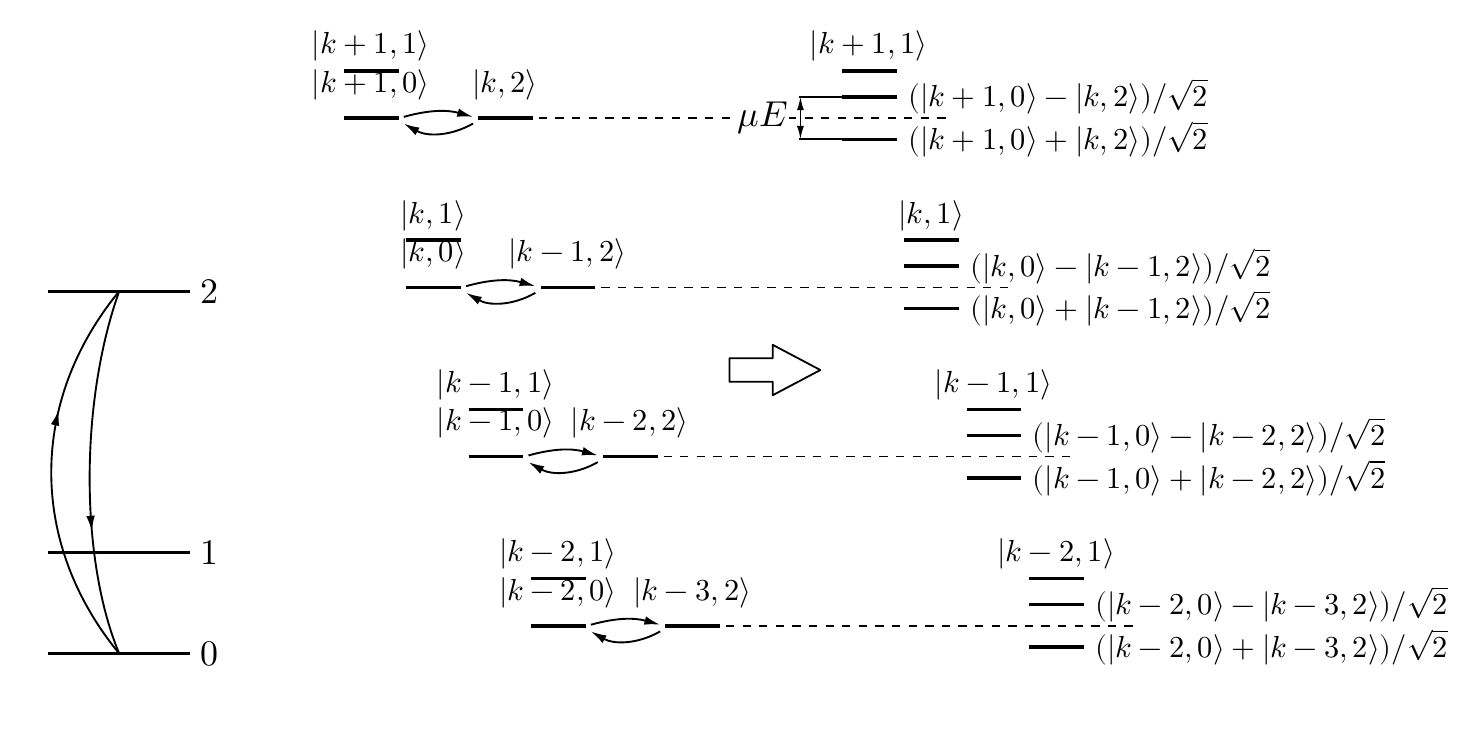
\begin{tikzpicture}[x=1cm,y=1cm,line join=round]
% At resonance: Q(k,0)=Q(k-1,2); gap=mu E. Real energies are schematic.
\coordinate (r0) at (1.05,1.3);\coordinate (r2) at (1.05,5.9);
\draw[lev] (.15,1.3)--(1.95,1.3) (.15,2.58372093)--(1.95,2.58372093) (.15,5.9)--(1.95,5.9);
\node[lab,anchor=west] at (2.03,1.3) {$0$};
\node[lab,anchor=west] at (2.03,2.58372093) {$1$};
\node[lab,anchor=west] at (2.03,5.9) {$2$};
\draw[flow] (r0) .. controls (-.1,2.7) and (-.1,4.5) .. (r2);
\draw[flow] (r2) .. controls (.55,4.5) and (.55,2.5) .. (r0);
\node[panel] at (1.05,.55) {а};
% The dressed-state panel receives extra horizontal room; no level energy changes.
\begin{scope}[xscale=1.10]
\draw[lev] (3.5500,8.1000)--++(0.6300,0);
\draw[lev] (5.1000,8.1000)--++(0.6300,0);
\draw[lev] (3.5500,8.7000)--++(0.6300,0);
\node[small,anchor=south] at (3.86,8.77) {$\lvert k+1,1\rangle$};
\node[small,anchor=south] at (3.86,8.28) {$\lvert k+1,0\rangle$};
\node[small,anchor=south] at (5.409999999999999,8.28) {$\lvert k,2\rangle$};
\draw[ray] (4.24,8.115) to[out=17,in=163] (5.04,8.115);
\draw[ray] (5.04,8.03) to[out=212,in=-32] (4.24,8.03);
\draw[fine,dashed] (5.8,8.1)--(10.55,8.1);
\draw[lev] (9.3000,8.3700)--++(0.6300,0);
\node[small,anchor=west] at (10.020000000000001,8.37) {$(\lvert k+1,0\rangle-\lvert k,2\rangle)/\sqrt{2}$};
\draw[lev] (9.3000,7.8300)--++(0.6300,0);
\node[small,anchor=west] at (10.020000000000001,7.83) {$(\lvert k+1,0\rangle+\lvert k,2\rangle)/\sqrt{2}$};
\draw[lev] (9.3000,8.7000)--++(0.6300,0);
\node[small,anchor=south] at (9.610000000000001,8.77) {$\lvert k+1,1\rangle$};
\draw[fine] (8.8,8.37)--(9.3,8.37) (8.8,7.83)--(9.3,7.83);
\draw[dimension] (8.82,7.83)--(8.82,8.37);\node[lab,anchor=east,fill=white] at (8.700000000000001,8.1) {$\mu E$};
\draw[lev] (4.2700,5.9500)--++(0.6300,0);
\draw[lev] (5.8200,5.9500)--++(0.6300,0);
\draw[lev] (4.2700,6.5500)--++(0.6300,0);
\node[small,anchor=south] at (4.579999999999999,6.619999999999999) {$\lvert k,1\rangle$};
\node[small,anchor=south] at (4.579999999999999,6.129999999999999) {$\lvert k,0\rangle$};
\node[small,anchor=south] at (6.129999999999999,6.129999999999999) {$\lvert k-1,2\rangle$};
\draw[ray] (4.959999999999999,5.964999999999999) to[out=17,in=163] (5.76,5.964999999999999);
\draw[ray] (5.76,5.879999999999999) to[out=212,in=-32] (4.959999999999999,5.879999999999999);
\draw[fine,dashed] (6.52,5.949999999999999)--(11.270000000000001,5.949999999999999);
\draw[lev] (10.0200,6.2200)--++(0.6300,0);
\node[small,anchor=west] at (10.740000000000002,6.219999999999999) {$(\lvert k,0\rangle-\lvert k-1,2\rangle)/\sqrt{2}$};
\draw[lev] (10.0200,5.6800)--++(0.6300,0);
\node[small,anchor=west] at (10.740000000000002,5.68) {$(\lvert k,0\rangle+\lvert k-1,2\rangle)/\sqrt{2}$};
\draw[lev] (10.0200,6.5500)--++(0.6300,0);
\node[small,anchor=south] at (10.330000000000002,6.619999999999999) {$\lvert k,1\rangle$};
\draw[lev] (4.9900,3.8000)--++(0.6300,0);
\draw[lev] (6.5400,3.8000)--++(0.6300,0);
\draw[lev] (4.9900,4.4000)--++(0.6300,0);
\node[small,anchor=south] at (5.3,4.47) {$\lvert k-1,1\rangle$};
\node[small,anchor=south] at (5.3,3.98) {$\lvert k-1,0\rangle$};
\node[small,anchor=south] at (6.849999999999999,3.98) {$\lvert k-2,2\rangle$};
\draw[ray] (5.68,3.815) to[out=17,in=163] (6.4799999999999995,3.815);
\draw[ray] (6.4799999999999995,3.73) to[out=212,in=-32] (5.68,3.73);
\draw[fine,dashed] (7.239999999999999,3.8)--(11.99,3.8);
\draw[lev] (10.7400,4.0700)--++(0.6300,0);
\node[small,anchor=west] at (11.46,4.07) {$(\lvert k-1,0\rangle-\lvert k-2,2\rangle)/\sqrt{2}$};
\draw[lev] (10.7400,3.5300)--++(0.6300,0);
\node[small,anchor=west] at (11.46,3.53) {$(\lvert k-1,0\rangle+\lvert k-2,2\rangle)/\sqrt{2}$};
\draw[lev] (10.7400,4.4000)--++(0.6300,0);
\node[small,anchor=south] at (11.05,4.47) {$\lvert k-1,1\rangle$};
\draw[lev] (5.7100,1.6500)--++(0.6300,0);
\draw[lev] (7.2600,1.6500)--++(0.6300,0);
\draw[lev] (5.7100,2.2500)--++(0.6300,0);
\node[small,anchor=south] at (6.02,2.3200000000000003) {$\lvert k-2,1\rangle$};
\node[small,anchor=south] at (6.02,1.8300000000000003) {$\lvert k-2,0\rangle$};
\node[small,anchor=south] at (7.569999999999999,1.8300000000000003) {$\lvert k-3,2\rangle$};
\draw[ray] (6.4,1.6650000000000003) to[out=17,in=163] (7.2,1.6650000000000003);
\draw[ray] (7.2,1.5800000000000003) to[out=212,in=-32] (6.4,1.5800000000000003);
\draw[fine,dashed] (7.96,1.6500000000000004)--(12.71,1.6500000000000004);
\draw[lev] (11.4600,1.9200)--++(0.6300,0);
\node[small,anchor=west] at (12.180000000000001,1.9200000000000004) {$(\lvert k-2,0\rangle-\lvert k-3,2\rangle)/\sqrt{2}$};
\draw[lev] (11.4600,1.3800)--++(0.6300,0);
\node[small,anchor=west] at (12.180000000000001,1.3800000000000003) {$(\lvert k-2,0\rangle+\lvert k-3,2\rangle)/\sqrt{2}$};
\draw[lev] (11.4600,2.2500)--++(0.6300,0);
\node[small,anchor=south] at (11.770000000000001,2.3200000000000003) {$\lvert k-2,1\rangle$};
\path[draw,line width=.65pt,fill=white] (8.0,5.05)--(8.5,5.05)--(8.5,5.22)--(9.05,4.90)--(8.5,4.58)--(8.5,4.75)--(8.0,4.75)--cycle;
\node[panel] at (10.0,.55) {б};
\end{scope}

\end{tikzpicture}
\end{document}
